\documentclass[research]{BMSTU-IU8}

\usepackage{amssymb} % triangleeq
\usepackage{pdfpages}

\student{Железцов Н.В.}
\theme{
    Разработка отказоустойчивой системы распределенных вычислений с
    использованием алгоритма консенсуса Raft
}
\group{ИУ8-104}

\supervisor{Колесников А.В.}

% \theme{Тест \hfill} % Тема для НИРСа заполняется по-другому
\studentFullName{Железцов Никита Владимирович}
\profile{20У474}
\speciality{10.05.01 <<Компьютерная безопасность>>}
\specialization{10.05.01\_01 <<Математические методы защиты информации>>}

\newacronym{bd}{БД}{База данных.}
\newacronym{subd}{СУБД}{Система управления базами данных.}
\newacronym{ddl}{DDL}{Data Definition Language.}
\newacronym{dql}{DQL}{Data Query Language.}
\newacronym{dml}{DML}{Data Manipulation Language.}
\newacronym{dcl}{DCL}{Data Control Language.}
\newacronym{lsn}{LSN}{Log sequence number.}
\newacronym{id}{ID}{Identifier.}
\newacronym{uuid}{UUID}{Universally unique identifier.}


\newglossaryentry{id1}{
    name={База данных (БД)},
    description={это организованная коллекция данных, которая структурирована таким образом, чтобы данные можно было легко хранить, управлять, изменять и извлекать.},
}

\newglossaryentry{id7}{
    name={Бакет},
    description={это логический контейнер, в который помещаются данные для
    распределения по шардам (физическим серверам или узлам). Это абстракция,
    которая связывает ключ шардирования с конкретным шардом.}
}

\newglossaryentry{id6}{
    name={Кластер},
    description={это совокупность нескольких репликасетов, каждый из которых чаще всего хранит разный набор данных.}
}

\newglossaryentry{id11}{
    name={Ребалансировка},
    description={процесс перевозки бакетов с одного шарда на другой.}
}

\newglossaryentry{id5}{
    name={Репликасет (replicaset, набор реплик, шард)},
    description={это группа узлов, работающих в режиме репликации и объединенных для обеспечения отказоустойчивости и доступности данных.}
}

\newglossaryentry{id2}{
    name={Система управления базами данных (СУБД)},
    description={это программное обеспечение, предназначенное для создания, управления и обеспечения доступа к базам данных. Оно позволяет пользователям определять, создавать, изменять и управлять базой данных, а также обеспечивает взаимодействие между пользователями и базой данных через запросы и команды. Основные функции включают хранение, поиск, обновление и удаление данных, а также обеспечение целостности, безопасности и управления доступом к данным.}
}

\newglossaryentry{id4}{
    name={Спейс (space)},
    description={это основная логическая единица хранения данных Tarantool, аналогичная таблице в традиционных реляционных базах данных. Спейс содержит набор записей, каждая из которых называется кортежем (tuple). Структура спейса определяется схемой, которая включает количество и типы полей в кортежах, а также индексы для быстрого доступа к данным.}
}

\newglossaryentry{id10}{
    name={Шардирование},
    description={это принцип проектирования базы данных, при котором данные
    разбиваются на части и размещаются на разных наборах реплик (репликасеты,
    шарды).}
}

\newglossaryentry{id8}{
    name={LSN},
    description={это монотонно возрастающий идентификатор записи.}
}

\newglossaryentry{id9}{
    name={Vclock},
    description={это массив LSN, идентификаторами в котором являются ID узлов. Vclock представляет собой набор логических счетчиков для каждого узла в кластере, позволяя определить, какие изменения были применены на конкретном узле и какие еще предстоит синхронизировать.}
}


\addbibresource{report.bib}

\begin{document}
    % \maketitle % Титульный лист

    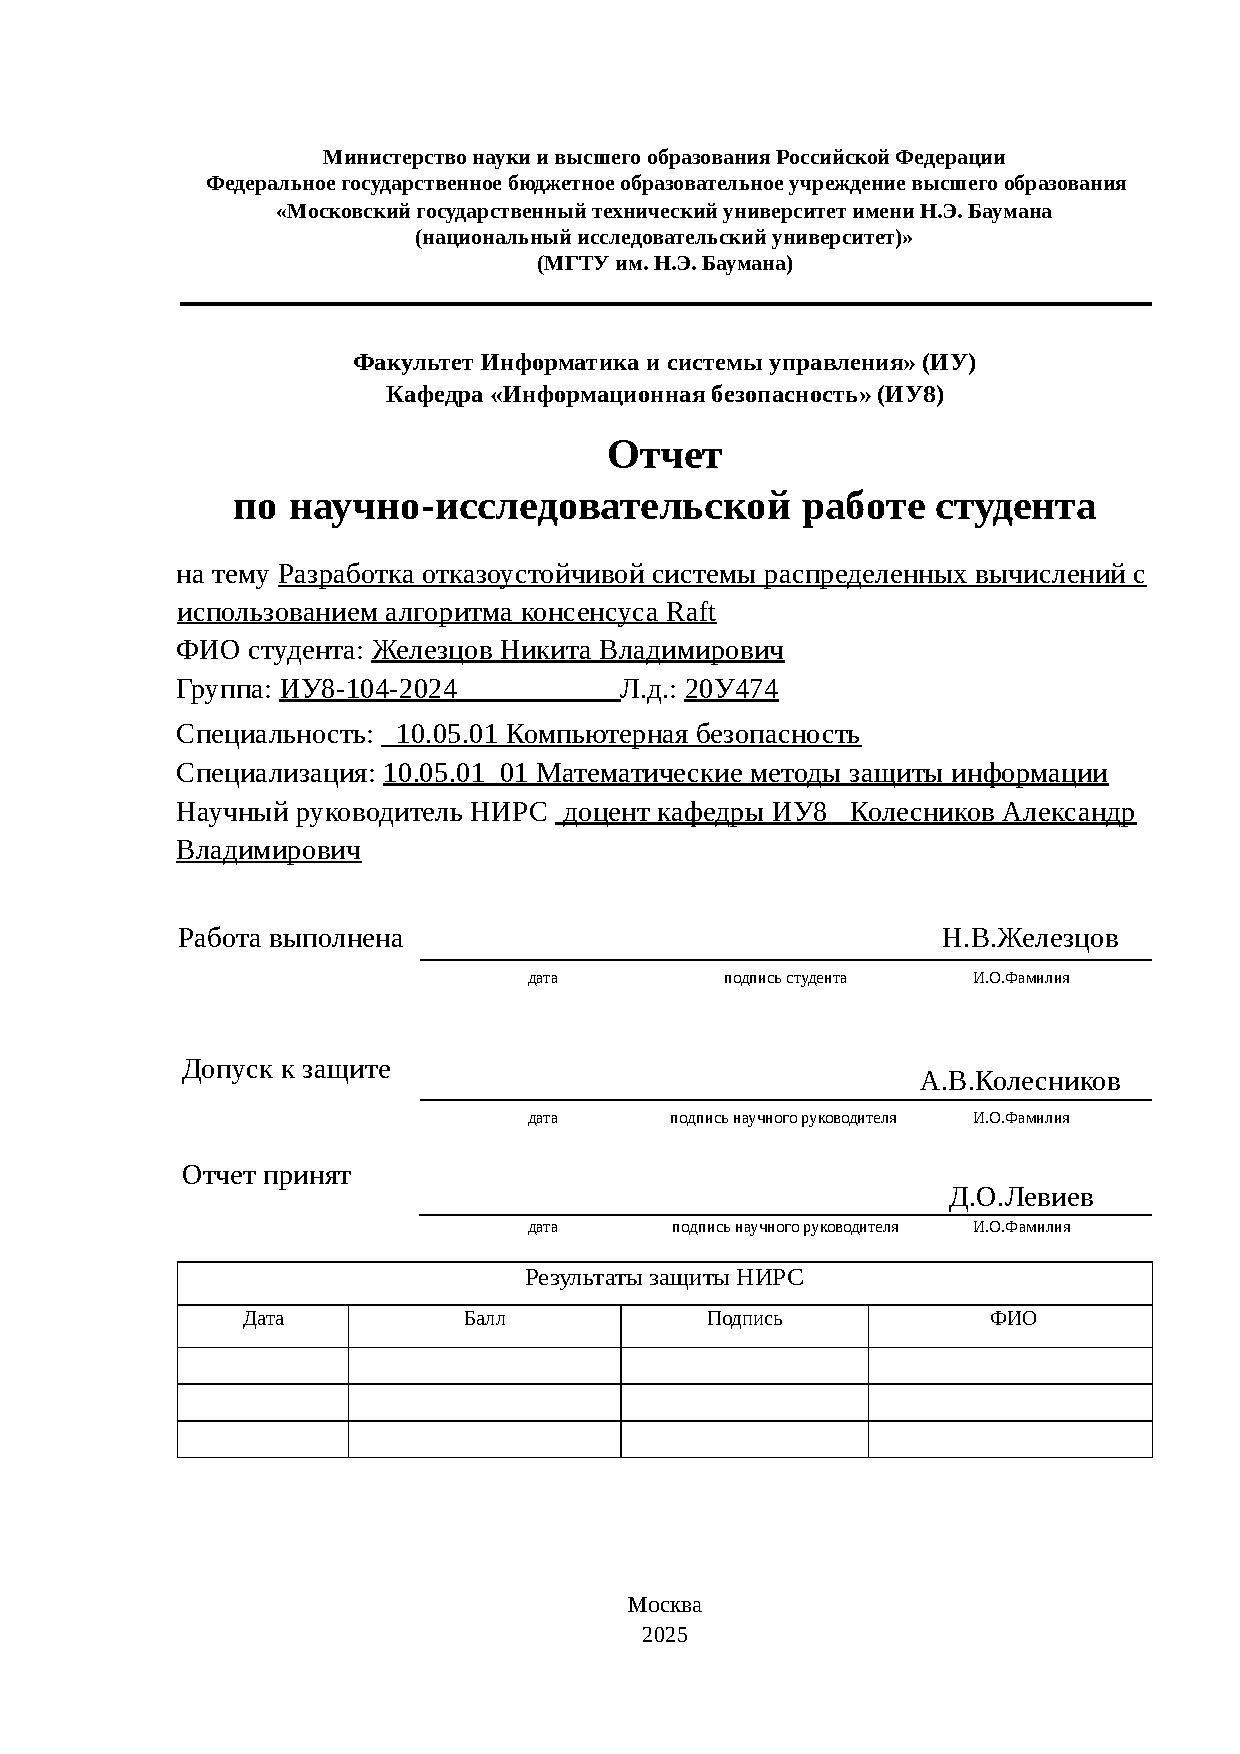
\includepdf[pages=-]{inc/titul.pdf} % Задание
    \setcounter{page}{4} % Устанавливает счётчик страниц

    \structure{РЕФЕРАТ}

Алгоритм Шора серьёзно поставил под вопрос безопасность информации, основанную
на криптосистемах с открытым ключом. Однако для взлома широко используемой
схемы RSA-2048 требуются миллионы физических кубитов, что значительно превышает
текущие технические возможности. Здесь мы сообщаем об универсальном квантовом
алгоритме факторизации целых чисел, объединяющем классическую редукцию базиса
решетки с квантовым алгоритмом приближённой оптимизации (QAOA). Количество
требуемых кубитов равно $O(\log N / \log\log N)$, что сублинейно относительно
битовой длины целого числа $N$, делая этот алгоритм самым экономичным по числу
кубитов алгоритмом факторизации на сегодняшний день. Мы экспериментально
демонстрируем алгоритм, факторизуя целые числа размером до 48 бит с помощью 10
сверхпроводящих кубитов, что является наибольшим целым числом, факторизованным
на квантовом устройстве. Мы оцениваем, что квантовая схема с 372 физическими
кубитами и глубиной в тысячи операций необходима для того, чтобы бросить вызов
RSA-2048 при помощи нашего алгоритма. Наше исследование демонстрирует
значительные перспективы для ускорения применения текущих шумных квантовых
компьютеров и прокладывает путь к факторизации больших целых чисел, имеющих
реальное криптографическое значение.
 % Реферат

    \tableofcontents % Содержание
    % \termsanddefenitions % Термины и определения
    % \listofabbreviations % Перечень сокращений и обозначений

    \structure{ВВЕДЕНИЕ}

Квантовые вычисления вступили в эпоху шумных квантовых устройств промежуточного
масштаба (NISQ) \cite{cite_1, cite_2}. Важной задачей эпохи NISQ является
демонстрация того, что устройства NISQ могут превзойти классические компьютеры
при решении задач с практической значимостью, то есть достижение практического
квантового преимущества. Алгоритмы, требующие минимальных ресурсов и
использующие ограниченное число доступных кубитов и глубину схем для решения
задач, сложных для классических вычислений, имеют особую важность. Вариационные
квантовые алгоритмы, использующие гибридную схему вычислений
«классика+квантовые вычисления», обладают значительным потенциалом для
получения значимого квантового преимущества в эпоху NISQ \cite{cite_3, cite_4,
cite_2, cite_5, cite_6}. Одним из таких алгоритмов является квантовый алгоритм
приближённой оптимизации (QAOA) \cite{cite_5}, первоначально предложенный для
решения задач на собственные значения, который впоследствии широко применялся в
различных областях, таких как химическое моделирование \cite{cite_7, cite_8},
машинное обучение \cite{cite_9}, а также инженерные приложения \cite{cite_10,
cite_11}.

Факторизация целых чисел является одной из важнейших основ современной
информационной безопасности \cite{cite_12}. Экспоненциальное ускорение
факторизации алгоритмом Шора \cite{cite_13} является выдающимся примером
превосходства квантовых вычислений. Однако выполнение алгоритма Шора на
отказоустойчивом квантовом компьютере требует значительных ресурсов
\cite{cite_14, cite_15}. На сегодняшний день наибольшее целое число,
факторизованное алгоритмом Шора на существующих квантовых системах, это число
21 \cite{cite_16, cite_17, cite_18}. Альтернативно, факторизация целых чисел
может быть сведена к задаче оптимизации, решаемой посредством адиабатических
квантовых вычислений (AQC) \cite{cite_19, cite_20, cite_21, cite_22} или QAOA
\cite{cite_23}. Более крупные числа были факторизованы этими методами на
различных физических системах \cite{cite_24, cite_25, cite_26, cite_27}.
Максимальные числа, факторизованные на данный момент, включают 291311 (19 бит)
в системе NMR \cite{cite_26}, 249919 (18 бит) на квантовом отжигателе D-Wave
\cite{cite_25}, 1099551473989 (41 бит) на сверхпроводящем устройстве
\cite{cite_27}. Однако следует отметить, что некоторые из факторизованных чисел
были специально подобраны с особыми структурами \cite{cite_28}, поэтому
наибольшее число, факторизованное универсальным методом на реальной физической
системе, на сегодняшний день составляет 249919 (18 бит).

В данной работе мы предлагаем универсальный квантовый алгоритм факторизации
целых чисел, требующий лишь сублинейные квантовые ресурсы. Алгоритм основан на
классическом алгоритме Шнорра \cite{cite_29, cite_30}, использующем редукцию
базиса решётки для факторизации целых чисел. Мы используем QAOA для оптимизации
наиболее трудоёмкой части алгоритма Шнорра, что ускоряет общее время
факторизации. Для целого числа $N$, имеющего $m$ бит, количество требуемых
кубитов в нашем алгоритме составляет $O(m / \log m)$, что сублинейно
относительно битовой длины числа $N$. Это делает наш алгоритм наиболее
экономным по числу кубитов по сравнению с существующими алгоритмами, включая
алгоритм Шора. С использованием данного алгоритма нами успешно факторизованы
числа 1961 (11 бит), 48567227 (26 бит) и 261980999226229 (48 бит) с
использованием, соответственно, 3, 5 и 10 кубитов на сверхпроводящем квантовом
процессоре. Число в 48 бит (261980999226229) также является наибольшим целым
числом, факторизованным универсальным методом на реальном квантовом устройстве.
Далее мы оцениваем квантовые ресурсы, необходимые для факторизации RSA-2048.
Согласно нашим расчётам, квантовая схема с 372 физическими кубитами и глубиной
порядка тысяч операций необходима для факторизации RSA-2048 даже в самой
простой одномерной системе. Подобный масштаб квантовых ресурсов, вероятно,
станет достижимым на устройствах NISQ в ближайшем будущем.

 % Введение

    \include{contents/2-00-analysys-of-the-subject}
    \section{Raft}

В Raft каждый узел хранит локально журнал команд, исполняемых конечным автоматом.
Так как все процессы получают одинаковые входные данные и применяют идентичные
команды в одном и том же порядке, их конечные автоматы приходят к одинаковому
состоянию. Одно из отличий Raft заключается в том, что роль лидера здесь
вынесена на первый план: он координирует репликацию и манипуляции над конечным
автоматом. С этой точки зрения Raft схож с Мульти-Паксосом и атомарной рассылкой:
среди узлов выбирается лидер, который принимает решения и задаёт упорядочение
сообщений.

Алгоритм Raft определяет три основные роли:

\begin{itemize}
    \item Кандидат (candidate): Узел, который пытается стать лидером. Он набирает
        голоса большинства узлов. Если выборы не приводят к явному победителю,
        запускается новый период и процесс голосования повторяется.
    \item Лидер (leader): Временный управляющий кластером, обрабатывающий запросы
        клиентов и взаимодействующий с реплицируемым конечным автоматом. Лидер
        выбирается на определённый период, который идентифицируется возрастающим
        номером. Если лидер перестаёт отвечать или подозревается в отказе,
        начинается процедура переизбрания.
    \item Последователь (follower): Пассивный участник, хранящий записи журнала
        и реагирующий на запросы от лидера и кандидатов. По сути, в Raft он
        объединяет в себе функции акцептора и ученика из Паксоса. Каждый узел
        стартует в роли последователя.
\end{itemize}

Чтобы добиться упорядочения без жёсткой синхронизации часов, в Raft используются
периоды (эпохи, термы), в течение которых существует только один лидер. Каждый
период имеет уникальный номер, а команды внутри периода получают дополнительный
индекс. Узлы могут по-разному воспринимать текущий период (например, если они
пропустили этап выборов), но каждая отправляемая команда указывает номер
периода \cite{ongario2014}. Если узел видит период с более высоким номером, он
обновляет своё значение периода.

Процесс выбора лидера инициируется, когда последователь не получает подтверждений
от текущего лидера, полагая, что тот вышел из строя. В этом случае последователь
переходит в состояние кандидата и собирает голоса большинства узлов, стремясь
стать новым лидером.

На рис. \ref{fig:raft} приведена схема раунда Raft.

\begin{figure}
  \centering
  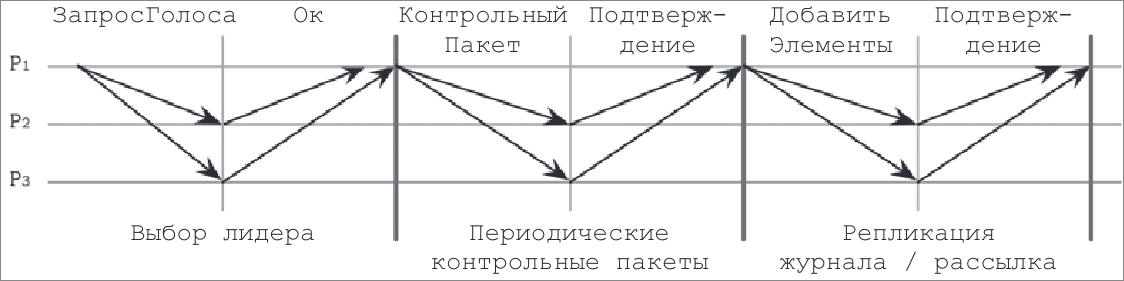
\includegraphics[scale=0.4]{inc/raft.png}
  \caption{Схема раунда Raft}
  \label{fig:raft}
\end{figure}

\begin{itemize}
    \item Выбор лидера. Когда узел-кандидат (P1 на рисунке) решает стать лидером,
        он рассылает остальным участникам сообщение $ЗапросГолоса$, содержащее свой
        период, последнюю известную ему информацию о периоде, а также идентификатор
        самой свежей записи в журнале, которую он видел. Если кандидат получает
        большинство голосов, он становится лидером на текущий период. При этом
        каждый узел может отдать голос лишь одному кандидату.
    \item Периодические контрольные пакеты. Для поддержания жизнеспособности
        системы лидер с определённой периодичностью отправляет контрольные
        пакеты всем последователям, тем самым подтверждая своё лидерство. Если
        последователь не получает такие пакеты в течение «тайм-аута выборов»,
        он предполагает сбой лидера и инициирует новый процесс голосования.
    \item Репликация. Лидер может неоднократно пополнять реплицируемый журнал,
        отправляя сообщение $ДобавитьЭлементы$, где указывает период лидера,
        индекс и период последней зафиксированной записи, а также одну или
        несколько новых записей для сохранения.
\end{itemize}

\subsection{Роль лидера в Raft}

Лидер может быть выбран только среди узлов, содержащих все актуальные записи.
Если в процессе выборов журнал последователя более актуальный, чем у кандидата,
то голос за этого кандидата не отдается.

Для победы в голосовании кандидат должен получить большинство голосов. Поскольку
записи реплицируются строго по порядку, достаточно сравнить идентификаторы последних
записей. После избрания лидер начинает принимать запросы от клиентов и реплицирует
их на своих последователей. Для этого он добавляет запись в свой журнал и
одновременно отправляет её всем последователям.

Когда последователь получает сообщение о добавлении записей, он вносит эти
записи в локальный журнал и отправляет подтверждение, сообщая лидеру, что данные
сохранены. Как только лидер получает достаточное количество подтверждений, запись
считается зафиксированной и помечается соответствующим образом в его журнале.

Поскольку лидером может стать только узел с наиболее актуальными данными,
последователь не отправляет ему обновления. Записи журнала передаются
только в одном направлении — от лидера к последователям.

На рисунке \ref{fig:raft-consensus} представлен пример раунда достижения
консенсуса, в котором узел P1 выступает в роли лидера с наиболее актуальной
информацией. Лидер выполняет алгоритм, реплицируя записи на своих последователей
и фиксируя их после получения подтверждений. Фиксация одной записи автоматически
фиксирует все предшествующие записи в журнале. Решение о фиксации может принимать
только лидер. Каждая запись в журнале имеет идентификатор периода (терма, указан в
верхнем правом углу записи) и индекс, определяющий её позицию в журнале.
Зафиксированные записи гарантированно реплицируются на кворум узлов, что
позволяет безопасно применять их к конечному автомату в порядке их добавления.

\begin{figure}
  \centering
  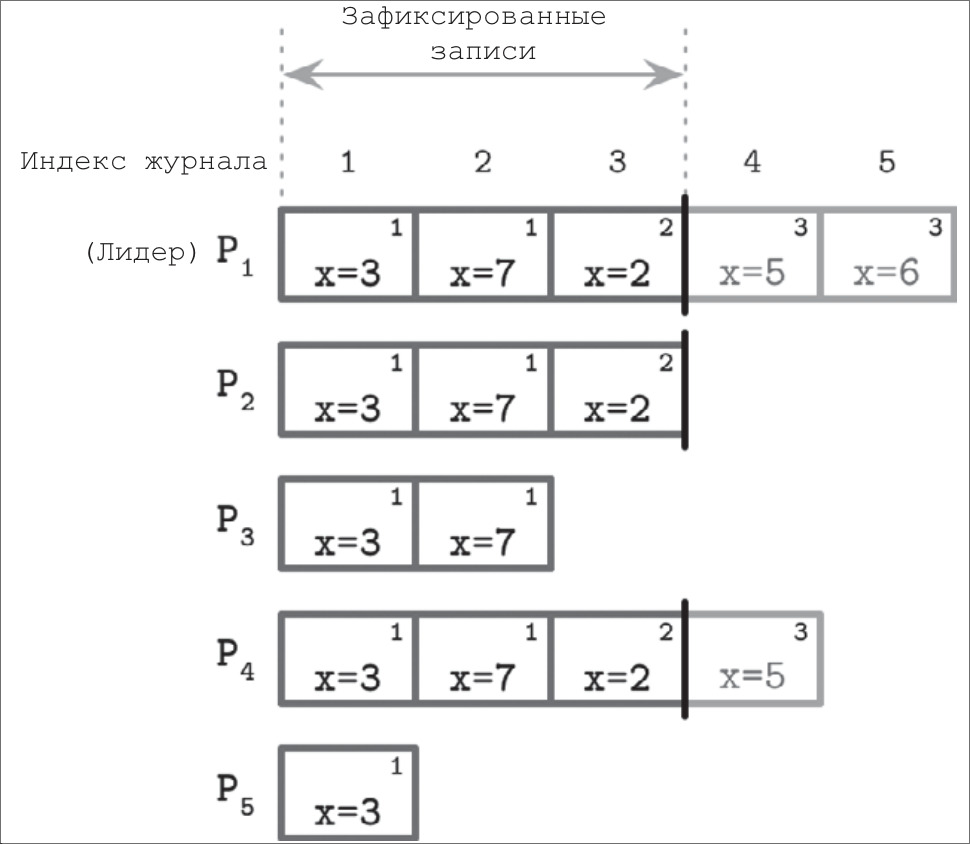
\includegraphics[scale=0.4]{inc/raft-consensus.png}
  \caption{Конечный автомат алгоритма Raft}
  \label{fig:raft-consensus}
\end{figure}

\subsection{Сценарии отказов}

Когда несколько последователей решают стать кандидатами, но ни один из них не
может набрать большинство голосов, такая ситуация называется "разделенным
голосованием". Чтобы снизить вероятность таких случаев, алгоритм Raft применяет
рандомизированные таймеры. Это позволяет одному из кандидатов начать следующий
этап выборов раньше других, получить достаточное количество голосов и быть
избранным, пока остальные кандидаты находятся в ожидании. Такой подход ускоряет
процесс выборов, исключая необходимость дополнительной координации между кандидатами.

Если последователи отключаются или задерживают ответы, лидер обязан
предпринимать дополнительные попытки доставки сообщений. Если подтверждение от
узлов не поступает в ожидаемый срок, лидер повторно отправляет сообщения.

Благодаря уникальным идентификаторам, присваиваемым реплицируемым записям,
порядок в журнале остается неизменным, даже при повторной доставке сообщений.
Последователи устраняют дублирующие записи, основываясь на их порядковых номерах,
что предотвращает нежелательные эффекты от повторных отправок. Также порядковые
номера используются для соблюдения хронологии в журнале: последователь отклоняет
записи с более высокими номерами, если предыдущие записи не совпадают с
его журналом. Если две записи из разных журналов имеют одинаковые идентификаторы
и индексы, то они хранят одну и ту же команду, а все предшествующие им записи
идентичны.

Для обнаружения сбоев лидер отправляет последовательным узлам контрольные
сообщения, подтверждая тем самым активность своего периода. Если один из узлов
замечает, что текущий лидер перестал отвечать, он инициирует процедуру выборов.
Новый лидер восстанавливает состояние кластера, определяя последнюю согласованную
запись (то есть запись с наибольшим номером, которую разделяют лидер и последователь).
Он приказывает узлам удалить все незафиксированные записи после этой точки и
реплицирует актуальные записи из своего журнала. Лидер не удаляет и не
перезаписывает собственные записи, а только добавляет новые.

Таким образом, Raft предоставляет следующие гарантии:

\begin{itemize}
    \item Только один лидер может быть избран одновременно на заданный период (терм);
        в течение одного периода не может быть двух активных лидеров;
    \item Лидер не удаляет и не переупорядочивает содержимое журнала; он только
        добавляет новые сообщения к нему;
    \item Зафиксированные записи в журнале гарантированно присутствуют в журналах
        для последующих лидеров;
    \item Все сообщения однозначно идентифицируются по идентификаторам сообщений
        и периодов; ни текущий, ни последующие лидеры не могут повторно использовать
        один и тот же идентификатор для другой записи.
\end{itemize}



    \conclusion

В ходе прохождения практики был проведён комплексный анализ механизма
шардирования в СУБД Tarantool. Основное внимание было уделено изучению
архитектуры модуля \texttt{vshard}, принципов распределения данных и
обеспечения согласованности при выполнении операций в шардированном кластере.

Были рассмотрены и проанализированы существующие подходы к реализации
Map-Reduce запросов по репликам. В результате исследования выявлены ключевые
проблемы, связанные с обеспечением консистентности данных при выполнении
распределённых запросов, и предложена альтернативная реализация.

Практическая значимость работы заключается в:
\begin{itemize}
    \item Систематизации знаний о работе шардированного кластера Tarantool;
    \item Выявлении ограничений существующей реализации модуля \texttt{vshard};
    \item Разработке предложений по расширению функциональности для поддержки
        Map-Reduce операций по репликам.
\end{itemize}

Полученные результаты могут быть использованы для дальнейшего развития модуля
шардирования Tarantool и улучшения его безопасности. Проведённое исследование
демонстрирует важность комплексного подхода к проектированию распределённых
систем и необходимость тщательного анализа требований к согласованности данных.

Результаты работы подтверждают возможность реализации эффективного механизма
выполнения Map-Reduce запросов по репликам в шардированной среде с соблюдением
требований к консистентности данных и производительности системы.


    \printbibliography

    \appendix
    \appendixsection{Основы теории решёток}

В последние годы решётки служат алгоритмическим инструментом для решения
широкого круга задач в информатике, математике и криптографии, особенно в
квантовоустойчивых криптографических протоколах. Ниже приведены базовые понятия
и известные алгоритмы, тесно связанные с нашей работой.

\subsection*{Базовые понятия}

Пусть $\lVert\cdot\rVert$ — евклидова норма векторов из $R^{m}$. Векторы
отмечаем полужирным (в переводе этого нет), матрицы пишем построчно; элементы
матрицы $M$ обозначаем $m_{i,j}$. Верхний индекс~$T$ — транспонирование.

\begin{itemize}
\item \textbf{Решётка.} Пусть $b_{1},\ldots,b_{n}\in R^{m}$ — линейно
        независимые столбцы, тогда множество всех линейных комбинаций их
        целочисленных коэффициентов — решётка, определяемая как
        \begin{equation} \Lambda(B) =\{\,Bx \mid x\in Z^{n}\,\} =\{\,b =
            x_{1}b_{1}+\dots+x_{n}b_{n} \mid x_{1},\dots,x_{n}\in Z\,\}.
        \end{equation} где $B=[b_{1},\ldots,b_{n}]\in R^{m\times n}$ — матрица
        базиса, которая также может быть использована чтобы представлять
        решетку для простоты. $\{b_1, \ldots, b_n\}$ - группа базиса решетки.
        Размерность решётки $n$. Её детерминант $\det\Lambda=(\det
        B^{T}B)^{1/2}$, здесь $B^T$ - транспонированная матрица $B$. При
        квадратной $B$ имеем $\det\Lambda=\det B$. Детерминант представляет
        объём решётки в геометрическом представлении, обозначается как
        $\operatorname{vol}(\Lambda)$. Длина точки $b\in R^{m}$ определяется
        как $\lVert b\rVert=(b^{T}b)^{1/2}$.

\item \textbf{Последовательные минимумы.} Для $n$‑мерной решётки $\Lambda$
        положительные числа $\lambda_{1}(\Lambda)\le\lambda_{2}(\Lambda)
        \le\dots\le\lambda_{n}(\Lambda)$ называются последовательными
        минимумами, где $\lambda_{k}(\Lambda)$ — наименьший радиус шара с
        центром в нуле, содержащего $k$ линейно независимых векторов из
        $\Lambda$. Обозначим $\lambda_{1}=\lambda_{1}(\Lambda)$ как длину
        кратчайшего ненулевого вектора из $\Lambda$.

\item \textbf{Постоянная Эрмита.} Эрмитовым инвариантом решётки $\Lambda$
        называется
        \begin{equation}
          \gamma(\Lambda)
          = \frac{\lambda_{1}^{2}(\Lambda)}{\operatorname{vol}(\Lambda)^{2/n}}
          = \frac{\lambda_{1}^{2}(\Lambda)}{\det(\Lambda)^{2/n}}.
        \end{equation}

        Постоянная Эрмита $\gamma_{n}$ — максимальное значение $\gamma(\Lambda)$
        для всех $n$‑мерных решёток, или минимальное константное $\gamma$,
        удовлетворяющее $\lambda_{1}(\Lambda)^{2}\le\gamma(\det\Lambda)^{2/n}$
        для всех решёток размености $n$ соответственно.

\item \textbf{QR‑разложение.} У решёточной матрицы базиса $B$ есть единственное
        разложение $B=QR\in R^{m\times n}$, где $Q\in R^{m\times n}$,
        $R=[r_{i,j}]_{1\le i,j\le n} \in R^{n\times n}$, здесь $Q\in R^{m\times
        n}$ — изомет­рическая (столбцы ортогональны и единичной длины), а $R
        \in R^{n\times n}$ — верхнетреугольная матрица с положительными
        диагональными элементами $r_{i,i}$. Коэффициенты Грама–Шмидта
        $\mu_{j,i}=r_{i,j}/r_{i,i}$ легко вычисляются из QR‑разложения. Для
        целочисленной $B$ коэффициенты $\mu_{j,i}$ обычно рациональны.

\item \textbf{Задача кратчайшего вектора (SVP).}
      Дана группа базиса $B$ решётки $\Lambda$.

      \begin{itemize}
          \item Задача кратчайшего вектора (SVP): Требуется найти вектор
              $v\in\Lambda$, такой что $\lVert v\rVert=\lambda_{1}(\Lambda)$.
          \item Приближённая задача кратчайшего вектора ($\alpha$‑SVP): Найти
              ненулевой вектор $v\in\Lambda$, удовлетворяющий
              $\lVert v\rVert\le\alpha\,\lambda_{1}(\Lambda)$.
          \item Эрмитова задача кратчайшего вектора ($r$‑Hermite SVP):
              Найти ненулевой вектор $v\in\Lambda$, такой что
              $\lVert v\rVert \;\le\; r\,\det(\Lambda)^{1/n}$.
      \end{itemize}

      Параметр $\alpha\ge1$ в $\alpha$‑SVP называется фактором аппроксимации.
      Обычнро задача упрощается при увеличении $\alpha$. При $\alpha=1$ задачи
      $\alpha$‑SVP и SVP совпадают. Истинное значение $\lambda_{1}$ в
      $\alpha$‑SVP трудно вычислить из-за сложности SVP, поэтому решение
      $\alpha$‑SVP не всегда легко проверить. Задача $r$‑Hermite SVP является
      вычислимой (относительно просто вычислимой), она определяется величиной
      $\det(\Lambda)^{1/n}$ вместо $\Lambda_1$. В результате, мы можем лешко
      проверить решение, но не можем сравнить его с кратчайшим вектором.

\item \textbf{Задача ближайшего вектора (CVP)}
      Дана группа базиса $B$ решётки $\Lambda$ и целевой вектор
      $t\in\operatorname{span}(B)$.

      \begin{itemize}
          \item Задача ближайшего вектора (CVP): Найти вектор $v\in\Lambda$,
              такой что расстояние $\lVert v - t\rVert$ может быть минимизировано,
              т.е. $\lVert v - t\rVert = \operatorname{dist}(\Lambda,t)$.
          \item $\alpha$-приближенная задача ближайшего вектора ($\alpha$‑CVP):
              Найти вектор $v\in\Lambda$, такой что расстояние
              $\lVert v - t\rVert \le \alpha \times \operatorname{dist}(\Lambda,t)$
          \item $r$-приближенная задача ближайшего вектора (($r$‑AbsCVP):  Найти
              $v\in\Lambda$ такое, что $\lVert v - t\rVert \le r$.
      \end{itemize}

      Определения аналогичны случаям для SVP; параметр $\alpha\ge1$ в
      $\alpha$‑CVP играет ту же роль, что и в $\alpha$‑SVP. В $r$‑AbsCVP
      параметр $r$ может быть любым разумным значением, соизмеримым с
      $\operatorname{dist}(\Lambda,t)$, например $\det(\Lambda)^{1/n}$ в
      $r$‑Hermite SVP.
\end{itemize}

\subsection*{Алгоритм LLL}
\begin{algorithm}[htp!]
    \SetAlgoLined

    \KwData{базис решётки $\text{b}_1, \dots, \text{b}_n \in \text{Z}^m$, параметр $\delta$}
    \KwResult{$\delta$-LLL-редуцированный базис}

    \textbf{Шаг 1:} Орторгонализация Грама-Шмидта \\
    Выполнить орторгонализацию Грама-Шмидта для базиса $\text{b}_1, \dots, \text{b}_n$, обозначим результат как $\tilde{\text{b}}_1, \dots, \tilde{\text{b}}_n \in \text{R}^m$

    \textbf{Шаг 2:} Редукция

    \For{$i = 2$; $i < n$; $i = i + 1$}{
        \For{$j = i-1$; $i > 1$; $ i = i - 1$}{
            $c_{i,j} = \left\lfloor \dfrac{\langle \text{b}_i, \tilde{\text{b}}_j \rangle}{\langle \tilde{\text{b}}_j, \tilde{\text{b}}_j \rangle} \right\rceil$; \\
            $\text{b}_i \gets \text{b}_i - c_{i,j} \cdot \text{b}_j$;
        }
    }

    \textbf{Шаг 3:} Обмен

    \If{$\exists \, i$ такое, что $\delta \cdot \| \tilde{\text{b}}_i \|^2 > \| \mu_{i+1,i} \tilde{\text{b}}_i + \tilde{\text{b}}_{i+1} \|^2$}{
        $\text{b}_i \leftrightarrow \text{b}_{i+1}$; \\
        перейти к шагу 1;
    }

    \textbf{Шаг 4:} Вывод базиса $\text{b}_1, \dots, \text{b}_n$

    \caption{Алгоритм LLL-редукции}
    \label{alg:lll}
\end{algorithm}

Алгоритм LLL — один из самых известных алгоритмов редукции решётки; он был
предложен А. К. Ленстрой, Х. В. Ленстрой (мл.) и Л. Ловашем в 1982 г.
\cite{cite_35}. Для $n$‑мерной решётки этот алгоритм позволяет решать $\alpha
\;=\; \left(\frac{2}{\sqrt{3}}\right)^{n}$ за полиномиальное время. Ниже
приведены связанные понятия и алгоритмы.

\newcounter{tmp-enum-lll}

\begin{itemize}
    \item \textbf{LLL базиc}: Базис $B = QR$ называется LLL‑редукции или
        LLL‑базисом при параметре редукции $\delta\in(1/4,1]$, если выполняются
        условия:
        \begin{enumerate}
            \item $\frac{\lvert r_{i,j}\rvert}{r_{i,i}} \;\le\; \frac12, \quad \text{for all } j > i;$
            \item $\delta\, r_{i,i}^{2}\;\le\;r_{i,i+1}^{2} + r_{i+1,i+1}^{2},\quad \text{for } i = 1,\ldots,n-1.$
            \setcounter{tmp-enum-lll}{\value{enumi}}
        \end{enumerate}

        Очевидно, LLL‑базис также удовлетворяет
        \( r_{i,i}^{2} \le \alpha\, r_{i+1,i+1}^{2} \),
        для \(\alpha = \frac{1}{(\delta - 1 / 4)}\).

        Параметры, рассматриваемые в оригинальной литературе по алгоритму LLL,
        равны $\delta = \tfrac34$, $\alpha = 2$. Известный результат о LLL‑базисе
        показывает, что для любого $\delta < 1$ LLL‑базис может быть получен за
        полиномиальное время и хорошо аппроксимирует последовательные минимумы\:

        \begin{enumerate}
            \setcounter{enumi}{\value{tmp-enum-lll}}
            \item $\alpha^{-\,i+1} \;\le\; \lVert b_{i}\rVert^{2}\,\lambda_{i}^{-2}
                \;\le\; \alpha^{\,n-1}, \quad \text{for } i = 1,\ldots,n;$
            \item $\lVert b_{1}\rVert^{2} \;\le\; \alpha^{\frac{n-1}{2}}\,
                \bigl(\det\Lambda\bigr)^{2/n}.$
        \end{enumerate}

    \item \textbf{Алгоритм LLL}: Для заданного набора базиса
        $B = [b_{1},\ldots,b_{n}] \in Z^{m\times n}$
        алгоритм может привести его к LLL‑редуцированному виду
        или преобразовать в LLL‑базис. Алгоритм состоит из трёх
        основных шагов: ортогонализация Грама–Шмидта, редукции и
        обмен. Конкретные шаги приведены в Алгоритме \ref{alg:lll}.
\end{itemize}

\subsection*{Алгоритм ближайшей плоскости Бабая}

Алгоритм ближайшей плоскости Бабая \cite{cite_32} (далее — алгоритм Бабая)
применяется для решения CVP. Для $n$‑мерной решётки он может получать фактор
аппроксимации $\alpha \;=\; 2\!\left(\frac{2}{\sqrt{3}}\right)^{n}$ для
$\alpha$‑CVP. Алгоритм состоит из двух этапов, первый из которых заключается в
редукции решетки с помощью алгоритма LLL. Второй является процедурой уменьшения
размера, который в основном вычисляет линейную комбинацию целочисленных
коэффициентов, ближайших к целевому вектору $t$ в LLL-базисе. Этот шаг по сути
совпадает со вторым шагом в LLL-редукции. Подробные действия приведены в
Алгоритме \ref{alg:babai}.

\begin{algorithm}[htp!]
    \SetAlgoLined

    \KwData{базис решётки $\text{b}_1, \dots, \text{b}_n \in \text{Z}^m$, параметр $\delta = 3/4$, целевой вектор $\text{t} \in \text{Z}^m$}
    \KwResult{вектор $\text{x} \in \Lambda(B)$, такой что $\|\text{x} - \text{t}\| \leq 2^{n/2} \, \text{dist}(\text{t}, \Lambda(B))$}

    \textbf{Шаг 1:} LLL-редукция \\
    Применить LLL-редукцию к базису $B$ с параметром $\delta$ \\
    Обозначим результат: $\tilde{\text{b}}_1, \dots, \tilde{\text{b}}_n \in \text{R}^m$

    \textbf{Шаг 2:} Уменьшение размера \\
    $\text{b} \gets \text{t}$

    \For{$j = n$; $j > 1$ $j = j-1$}{
        $c_j = \left\lfloor \dfrac{\langle \text{b}, \tilde{\text{b}}_j \rangle}{\langle \tilde{\text{b}}_j, \tilde{\text{b}}_j \rangle} \right\rceil$ \\
        $\text{b} \gets \text{b} - c_j \cdot \text{b}_j$
    }

    \textbf{Шаг 3:} Вернуть $\text{t} - \text{b}$

    \caption{Алгоритм Бабая}
    \label{alg:babai}
\end{algorithm}

    \appendixsection{Алгоритм Шнорра для факторизации целых чисел}

\subsection*{Метод решета Шнорра}

Рассмотрим общую задачу факторизации, в которой задано целое число $N$,
предполагается разложить его на два нетривиальных множителя $p<q$, так что $N =
p\times q$. Метод решета для факторизации начинается с определения пары гладких
отношений.

Пусть $p_i,\; i = 1,\dots,n$ — первые $n$ простых чисел вместе с $p_0$,
удовлетворяющими $-1 = p_0 < 1 < p_1 < \dots < p_n < p$. Множество $P =
\{p_i\}_{i=0,\dots,n}$ называется простым базисом. Число $p_0 = -1$ не является
простым, однако включается для учёта знака целого числа. Целое число называется
$p_n$‑гладким, если все его простые делители меньше $p_n$; число $p_n$ при этом
называют пределом гладкости. Пара целых чисел $(u_j,v_j)$ называется
$p_n$‑гладкой парой, если и $u_j$, и $v_j$ являются $p_n$‑гладкими. Более того,
пара целых чисел $(u_j,v_j)$ называется $p_n$‑гладкой парой отношений
(сокращённо sr‑пара), если:

\begin{equation}
  u_{j} \;=\; \prod_{i=1}^{n} p_{i}^{\,e_{i,j}},
  \qquad
  u_{j} - v_{j}N \;=\; \prod_{i=0}^{n} p_{i}^{\,e'_{i,j}},
\end{equation}

\noindent где $e_{i,j},\,e'_{i,j}\in{N}$, тогда имеем

\begin{equation}
  \frac{u_{j}-v_{j}N}{u_{j}}
  \;\equiv\;
  \prod_{i=0}^{n} p_{i}^{\,e'_{i,j}-e_{i,j}}
  \;\equiv\; 1 \pmod{N}.
\end{equation}

Следует отметить, что гладкая пара отличается от sr‑пары: sr‑пара должна не
только быть $p_n$‑гладкой, но и удовлетворять более строгим условиям в
уравнении Б.3. Пусть $S=\{(u_j,v_j)\}_{j=1,\dots,n+1}$ — набор из $n\!+\!1$
sr‑пар. Пусть существуют коэффициенты $ t_1,\dots,t_{n+1}\in\{0,1\}$, такие что:

\begin{equation}
  \sum_{j=1}^{n+1} t_{j}\bigl(e'_{i,j}-e_{i,j}\bigr)
  \;\equiv\; 0 \pmod{2},
  \qquad i = 0,1,\dots,n.
\end{equation}

\noindent Обозначим $X \;=\ \prod_{i=0}^{n}p_{i}^{\frac12 \sum_{j=1}^{n+1} t_{j}\bigl(e'_{i,j}-e_{i,j}\bigr)},$
тогда

\begin{equation}
  X^{2}-1 \;=\; (X+1)(X-1) \;\equiv\; 0 \pmod{N}.
\end{equation}

\noindent Если $X \not\equiv \pm1 \pmod{N}$, то нетривиальный фактор числа $N$
получается как $\gcd(X \pm 1,\, N)$.

Поскольку размерность системы линейных уравнений равна~$O(n)$ и она решается
за~$O(n^{3})$ операций, эту малую часть вычислений при факторизации~$N$ мы
опускаем. Следовательно, задача факторизации сводится к задаче поиска sr‑пары.
В дальнейшем эта задача будет преобразована в задачу ближайшего вектора на
решётке.

\subsection*{Построение решётки и целевого вектора}

sr‑пары будут получены из приближённого решения задачи CVP в алгоритме Шнорра.
Сначала опишем построение простой решётки $\Lambda(B_{n,c})$ и целевого вектора
$t\in \mathbb{R}^{\,n+1}$; здесь $c>0$ — настраиваемый параметр. Матрица решётки
$B_{n,c}=[b_{1},\dots,b_{n}]\in \mathbb{R}^{(n+1)\times n}$ задаётся

\begin{equation}
  B_{n,c} =
  \begin{pmatrix}
    f(1)      & 0        & \dots & 0        \\
    0         & f(2)     & \dots & 0        \\
    \vdots    & \vdots   & \ddots& \vdots   \\
    0         & 0        & \dots & f(n)     \\
    N^{c}\ln p_{1} & N^{c}\ln p_{2} & \dots & N^{c}\ln p_{n}
  \end{pmatrix},
  \qquad
  t =
  \begin{pmatrix}
    0 \\[2pt]
    \vdots \\[2pt]
    0 \\[2pt]
    N^{c}\ln N
  \end{pmatrix}.
\end{equation}

\noindent где функции $f(i)$ при $i=1,\dots,n$ — случайные перестановки
диагональных элементов $(\sqrt{\ln p_{1}},\sqrt{\ln p_{2}},\dots, \sqrt{\ln
p_{n}})$.

Точку решётки или вектор можно представить целочисленной комбинацией базиса
решетки: $b=\sum_{i=1}^{n} e_{i} b_{i}\in\Lambda(B_{n,c})$, причём $e_{i}\in
Z$. Далее будем полагать, что $(u,v)$ — $p_{n}$‑гладкая пара и $\gcd(u,v)=1$.
Тогда $u,v$ выражаются через произведение простых чисел из простого базиса:

\begin{equation}
  u \;=\; \prod_{e_{i}>0} p_{i}^{\,e_{i}},
  \qquad
  v \;=\; \prod_{e_{i}<0} p_{i}^{\,-e_{i}}.
\end{equation}

В таком представлении гладкой паре $(u,v)$ взаимно однозначно соответствует
вектор $b=(e_{1},\dots,e_{n})$ на решётке, пишем $b\sim(u,v)$. Таким образом,
вектор решётки кодирует гладкую пару.

Задача ближайшего вектора (CVP) формулируется как поиск вектора
$b_{0}\in\Lambda(B_{n,c})$, минимально удалённого от $t$:

\begin{equation}
    b_{0} \;=\; \arg\min_{\,b\in\Lambda}\;\lVert b - t\rVert.
\end{equation}

Согласно приведённому выше определению справедливо отношение:

\begin{equation}
  \lVert b - t\rVert^{2}
  \;\ge\;
  \ln(uv) \;+\; N^{2c}\,\bigl|\ln\tfrac{u}{vN}\bigr|^{2}.
\end{equation}

Уравнение выполняется тогда и только тогда, когда $e_{i}\in\{-1,0,1\}$, то есть
$u,v$ не содержат квадратных множителей. Константа $N^{2c}$ выступает «весом»,
управляемым параметром $c$. При $N^{2c}\gg\ln(uv)$ главной частью равенства
становится $N^{2c}\,|\ln\frac{u}{vN}|^{2}$. Следовательно, параметр $c$ (также
называемый параметром точности) влияет на величину $|\ln\frac{u}{vN}|^{2}$, а
значит и на $|u-vN|$. Из неравенства Б.10 видно: чем короче вектор расстояния
$b-t$, тем меньше $|u-vN|$ и тем выше вероятность того, что $(u,v)$ является
sr‑парой. Дополнительное обсуждение этой зависимости приведено в следующем
разделе материала.

\subsection*{Решение CVP}

Существует два хорошо изученных подхода к решению задачи ближайшего вектора
(CVP) или её аппроксимации. Первый основан на методе решета, впервые
предложенном Айтаем с соавторами в 2001 г. \cite{cite_36}. Второй базируется на
алгоритме Бабаи: сначала выполняют редукцию решётки (например, алгоритмом LLL),
чтобы получить относительно короткий базис, а затем применяют процедуру
уменьшения размера для получения приближённого решения CVP. Шнорр использовал
именно второй подход. Фактически для повышения эффективности алгоритма
привлекают более совершенные методы редукции, такие как BKZ \cite{cite_37},
HKZ, ENUM \cite{cite_37,cite_38,cite_39,cite_40} и др. Однако эти методы
слишком сложны и требуют специальных знаний, выходящих за рамки данной работы.
Поэтому далее (также и в основном тексте) под алгоритмом Бабаи мы будем
подразумевать реализацию с использованием LLL‑редукции, которая проста и
относительно легко понимается. При этом принцип квантового ускорения алгоритма
Бабаи остается общим для любого метода редукции решётки.

\end{document}
